\documentclass{beamer}
\usepackage{etex}
\usetheme{Antibes}
\usepackage{amssymb,amsmath,amsthm}
\usepackage{graphicx}
\usepackage{caption}
\usepackage{subfig}
\newcommand{\bn}{\begin{enumerate}[i)]}
\newcommand{\en}{\end{enumerate}}
\newcommand{\im}{\item}
\newcommand{\CPT}[1]{\large{\textbf{CHAPTER #1}}}
\newcommand{\ir}[1]{\textbf{Remark #1}}
\newcommand{\ith}[1]{\textbf{Theorem #1}}
\newcommand{\idf}[1]{\textbf{Definition #1}}
\newcommand{\iex}[1]{\textbf{Example #1}}

%\definecolor{cardinal}{rgb}{0.77, 0.12, 0.23}
%\usecolortheme[named=cardinal]{structure}
%\setbeamercolor{block title}{bg=cardinal,fg=black}
 \usepackage{tikz}
 \usetikzlibrary{patterns,snakes,plotmarks}
 \usepackage{multirow}
% \usetikzlibrary{shadows}
\usepackage{epstopdf}
\usepackage{nicefrac}
\usepackage{lmodern}
\usepackage{pgfplots}
\usepackage{qtree}
\newcommand*{\Scale}[2][4]{\scalebox{#1}{\ensuremath{#2}}}%
\DeclareCaptionLabelSeparator{horse}{:\,\,} % change according to your needs
\captionsetup{
  labelsep = horse,
  figureposition = bottom % used to get the correct vertical space between the figure and the caption
}
\setbeamertemplate{caption}[numbered]
\setbeamertemplate{items}[circle]
\setbeamertemplate{enumerate items}[square]
\theoremstyle{definition}
\newtheorem*{exs}{Examples}
\newtheorem{ex}{Example}
\newtheorem*{exc}{Exercise}
%\usepackage{booktabs}
\setlength{\parindent}{0pt}
%\setbeameroption{show notes}
 \setbeamerfont{note page}{size=\tiny}
%\setbeamertemplate{note page}[plain]
%\setbeameroption{show only notes}
\title{Math 629 - Survival Analysis \\ Chapter 7: Parametric Survival Models
}
\author{Drew Lazar}
\institute{Ball State University}
\date{\today}

\begin{document}
\begin{frame}
    \titlepage
\end{frame}



\section{Chapter 7}
\begin{frame}
\frametitle{Parametric Survival Models}
\begin{block}{Overview}
\begin{enumerate}
\item Explain parametric survival models, compare to semi-parametric and non-parametric models.
\item We explain the accelerated failure time assumption (AFT), the proportional odds assumption (PO) and compare to proportional hazard assumption (PH).
\item We present examples of several parametric models, including the exponential model, the Weibull model, and the
log-logistic model.
\item We discuss interval censored data modeled by parametric models.
\item We introduce frailty models which allow for flexibility in individual subjects in parametric models.
\end{enumerate}
\end{block}
\end{frame}

\begin{frame}
\frametitle{Parametric Survival Models}
\begin{block}{Definition and Explanation of Parametric Survival Models}
\begin{itemize}
\item In parametric survival models the outcome (survival) is from some family of
distributions of similar form with unknown parameters. When the value of the parameter(s) is known then the exact distribution
is fully specified.
\item A Cox PH model is semi-parametric as there are parameters involved but they do not fully specify the distribution.
\item Kaplan-Meirer estimates, log-rank statistics, overall hazards rates and survival times are non-parametric.
\end{itemize}
\end{block}
\end{frame}

\begin{frame}
\frametitle{Parametric Survival Models}
\begin{block}{Definition and Explanation of Parametric Survival Models}
\begin{itemize}
\item Parametric models typically require more assumptions then semi-parametric models. They are thus less ``robust''.
\item If assumptions are met then parametric models are preferable as they fully specify distribution.
\item The theoretical survival curve is smooth and so is the estimate from the parametric model. A semi-parametric or non-parametric model returns a step-function.
\end{itemize}
\vspace{-5pt}
\begin{center}
        \includegraphics[width=5cm, height=2.9cm]{CH7_pcurves.JPG}
    \end{center}
\end{block}
\end{frame}

\begin{frame}
\frametitle{Parametric Survival Models}
\begin{block}{The pdf, survival function and hazard function}
Recall:
\begin{align*}
& S(t) = P(T>t) \text{ and } h(t) = \lim_{\Delta t \rightarrow 0} \frac{P(t \le T < t + \Delta t | T \ge t)}{\Delta t} \\
& \text{ and we have the following relationship} \\
& S(t) = \exp\left[-\int_0^t h(u) du\right] \text{ and } h(t) = -\frac{d S(t)/dt}{S(t)}. \\
\end{align*}
\end{block}
\end{frame}

\begin{frame}
\frametitle{Parametric Survival Models}
\begin{block}{The pdf, survival function and hazard function (cont'd)}
The pdf of a survival distribution is the function $f(t)$ such that
\begin{align*}
& S(t) = \int_t^\infty f(t) dt \\
& \text{ Using the fundamental theorem of Calculus we have } \\
& \frac{-d(S(t))}{dt} = f(t) \text{ thus } h(t) = -\frac{d S(t)/dt}{S(t)} = \frac{f(t)}{S(t)} \\
\end{align*}
\end{block}
\end{frame}

\begin{frame}
\frametitle{Parametric Survival Models}
\begin{block}{Some parametric survival distributions}
\begin{center}
\begin{tabular}{ c c c c }
Distribution & $S(t)$ & $f(t)$ & $h(t)$  \\    \hline
Exponential  & $\exp(-\lambda t)$  & $\lambda \exp(-\lambda t)$ & $\lambda$    \\
Weibull      & $\exp(-\lambda t^p)$ & $ \lambda p t^{p-1} \exp(-\lambda t^p)$ & $\lambda p  t^{p-1}$  \\
Log-logistic & $\frac{1}{1 + \lambda t^p}$ & $\frac{\lambda p t^{p-1}}{(1+\lambda t^p)^2}$ & $\frac{\lambda p t^{p-1}}{(1+\lambda t^p)}$ \\ \hline
\end{tabular}
\end{center}
\end{block}
Typically, you will reparameterize in order to allow for the effect of covariates.
\end{frame}


\begin{frame}
\frametitle{Parametric Survival Models}
\begin{block}{Example 7.1 - Exponential Distribution}
Assume the population approximately follows the exponential distributions so that
\[
S(t;X) = \exp(-\lambda t) = \exp[-(\beta_0 + \beta_1 X)t]
\]
where $X$ is a single covariate. \\

You might have $\hat{\beta}_0=.2$ and $\hat{\beta}_1=.3$ so for $X=1$ you have
\[
\hat{S}(t;1) = \exp(-0.5 t)
\]
\begin{center}
        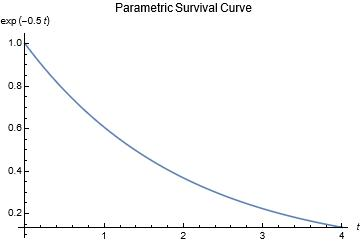
\includegraphics[width=5cm, height=2.1cm]{CH7_ex1.JPG}
    \end{center}
\end{block}
\end{frame}






 \begin{frame}
\frametitle{Parametric Survival Models}
\begin{block}{Definition 7.1 - Three properties of survival analysis populations}
Let $X$ and $X^*$ be any two different specifications of the covariates.
\begin{enumerate}
\item Proportional Hazards (PH)
\[ h(t;X)/h(t;X^*) = \theta \text{ for all } t>0, \text{ constant } \theta > 0 \]
\item Accelerated Failure Times (AFT)
\[ S(t;X) =  S(\gamma t;X^*)  \text{ for all } t>0, \text{ constant } \gamma > 0
\]
\item Proportional Odds (PO)
\[ \frac{1- S(t;X)}{S(t;X)} = \tau \left(\frac{1- S(t;X^*)}{S(t;X^*)}\right)  \text{ for all } t>0, \text{ constant } \tau > 0
\]
\end{enumerate}
\end{block}
\end{frame}


\begin{frame}
\frametitle{Parametric Survival Models}
\begin{block}{Assumptions of some parametric distributions }
\begin{center}
\begin{tabular}{ c c c | c }
Distribution & $S(t)$ & $h(t)$ & Accommodates \\ \hline
Exponential & $\exp(-\lambda t)$ & $\lambda$ & PH, AFT \\
Weibull  & $\exp(-\lambda t^p)$ & $\lambda p t^{p-1}$ & PH, AFT\\
Log-logistic & $\frac{1}{1+\lambda t^p}$ & $ \frac{\lambda p t^{p-1}}{1+\lambda t^p}$ & PO, AFT
\end{tabular}
\end{center}
\end{block}
We will show each of these.
\end{frame}

\begin{frame}
\frametitle{Parametric Survival Models}
\begin{block}{Illustration 1 of Accelerated Failure Time property}
It is said ``every dog year is seven human years''. So if $X=0$ is dogs and $X=1$ is humans then
\[
S(t,0) = S(7t,1) \text{ for any } t>0.
\]
\begin{center}
        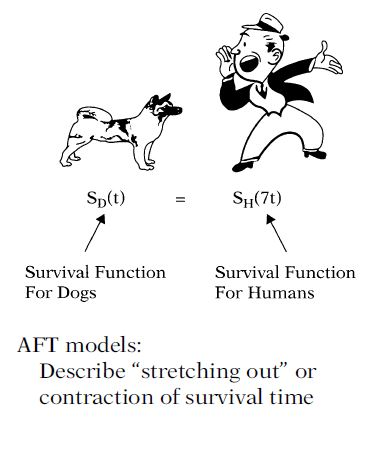
\includegraphics[width=5cm, height=4.5cm]{CH7_Dogs.JPG}
    \end{center}
\end{block}
\end{frame}

\begin{frame}
\frametitle{Parametric Survival Models}
\begin{block}{Illustration 2 of Accelerated Failure Time property}
Assume our survival random variable ($T$) is time to death of 60 years olds and $X$ is smoking status (0=non-smoker, 1=smoker).
Assume we have
\[
S(t;0) = S((2/3)t,1) \text{ for all } t>0
\]
Let $T_0$ be the survival random variable for non-smokers and $T_1$ be the survival random variable for smokers.

Then
\[ S(7.5;0) = P(T_0>7.5) = P(T_1>5;1) \]
 and
\[S(15;0) = P(T_0>15) = S(10;1) = P(T_1>10)
\]
Note we have $S((3/2)t;0) = S(t;1)$ and $T_1=(2/3)T_0$.
\end{block}
\end{frame}


\begin{frame}
\frametitle{Parametric Survival Models}
\begin{block}{Accelerated Failure Time property}
In general, if we have the AT property for some $\gamma$ so that
\[ S(t;X) =  S(\gamma t;X^*)  \text{ for all } t>0, \text{ constant } \gamma > 0
\]
then
 \[ S((1/\gamma)t;X) =  S( t;X^*)  \text{ for all } t>0, \text{ constant } \gamma > 0.
\]
and if $T_X$ and $T_{X^*}$ are respective conditional random variables then
\[
\gamma T_X = T_{X^*}
\]
\end{block}
\end{frame}

\begin{frame}
\frametitle{Parametric Survival Models}
\begin{block}{Exponential accommodates PH}
Exponential accommodates PH. Why? Let
\[
\lambda=\exp(\beta_0 + \beta' X)
\] where $\beta, X$ are both $p \times 1$.
Then
\[
\text{HR}(X \text{ vs. } X^*)  = \dfrac{\exp(\beta_0 + \beta' X)}{\exp(\beta_0 + \beta' X^*)} = \exp(\beta'(X - X^*))
\]
\end{block}
\end{frame}

\begin{frame}
\frametitle{Parametric Survival Models}
\begin{block}{Exponential accommodates AFT.}
Exponential accommodates AFT. Why? For any survival time $0 < q < 1$ solve
\begin{align*}
& q = S(t) = \exp(- \lambda t) \implies \ln(q) = - \lambda t \implies \\
& t = \frac{1}{\lambda} (- \ln(q)).
\end{align*}
Let
\[
\frac{1}{\lambda} = \exp(\alpha_0 + \alpha'X)
\]
Then $\exp(\alpha_0 + \alpha_1'X)(- \ln(q))$ is time to ``reach" $q$ for any $X$. Thus,
\vspace{-10pt}
\[
\gamma = \text{AF($X$ vs. $X^*$)} = \frac{\exp(\alpha_0 + \alpha'X)}{\exp(\alpha_0 + \alpha'X^*)} = \exp(\alpha'(X-X^*)).
\]
\end{block}
\end{frame}


\begin{frame}
\frametitle{Parametric Survival Models}
\begin{block}{Relationship between AF and HR for exponential model}
Relationship between AF and HR for exponential model. We have
\[
\lambda = \exp(\beta_0 + \beta'X) \text{ and } \frac{1}{\lambda} = \exp(\alpha_0 + \alpha'X)
\]
Thus,
\[ \ln(\lambda) = \beta_0 + \beta'X = -\alpha_0 - \alpha'X \implies \beta_0 = -\alpha_0 \text{ and } \beta'=-\alpha' \]
Thus,
\begin{align*}
&\theta = \text{HR}(X \text{ vs. } X^*) = \exp(\beta'(X - X^*)) =\\
&\exp(-\alpha'(X - X^*)) = 1/\text{AF}(X \text{ vs. } X^*) = 1/\gamma.
\end{align*}
\end{block}
\end{frame}

\begin{frame}{Example 7.2 - Modeling Remission Data w/Exponential Model}
\begin{block}{Remission Data}
\begin{enumerate}[ ]
\item Remission data ($n=42$). Covariate treatment status (TR).
\item 21 given treatment (TR=1). 21 given placebo (TR=0).
\end{enumerate}
\end{block}
\begin{block}{As a PH model}
Assuming an exponential distribution, we parameterize
\[ h(t;TR)= \lambda = \exp(\beta_0 + \beta_1 TR)
\]
We have hazard ratio
\[
\text{ HR(TR=0 vs. TR=1) } = \exp(\beta_1)
\]
 \end{block}
 \end{frame}

\begin{frame}{Example 7.2 - Modeling Remission Data w/Exponential Model, cont'd}
\begin{block}{As a AFT model}
Assuming an exponential distribution, we parameterize
\[ \frac{1}{\lambda} = \exp(\alpha_0 + \alpha_1 TR)
\]
We have AF factor
\[
\text{ AF(TR=0 vs. TR=1) } = \exp(\alpha_1)
\]
 \end{block}
 \end{frame}

 \begin{frame}{Modeling Remission Data w/Exponential Model}
\begin{block}{Problem 7.1 - Modeling the Remission Data with an exponential model}
\begin{enumerate}
\item Fit an AFT exponential model to the Remission data using only covariate TR.
\begin{enumerate}[i.]
\item Give the fitted model and the AF for TR. Give $95\%$ CI for AF.
\item Give fitted PH model and the HR  for TR. Give $95\%$ CI for HR.
\end{enumerate}
\item Fit an AFT exponential model to the Remission data using covariates TR and LogWBC.
\begin{enumerate}[i.]
\item Give fitted model and the AF for TR. Give $95\%$ CI for AF.
\item Give fitted PH model and the HR for TR. Give $95\%$ CI for the AF.
\item Add an interaction term to your AFT model. Is this interaction significant?
\item Under interaction give the HR and AF for TR at quartiles of logWBC.
\end{enumerate}
\end{enumerate}
 \end{block}
 \end{frame}

\begin{frame} 
\frametitle{Parametric Survival Models}\
\begin{block}{Weibull Model} 
\begin{itemize}
\item Most widely used parametric model 
\item It's hazard function is given
\[ h(t) = \lambda p t^{p-1} \text{ with } p>0, \lambda >0 
\]
\item $p$ is known as the shape parameter. 
\begin{itemize}
\item If $p>1$ hazard increases over time
\item If $p=1$ constant hazard (exponential model)
\item If $p<1$ hazard decreases over time
\end{itemize}
\item Typically $\lambda$ is parameterized to account for covariates and $p$ is fixed.
\item With $p$ fixed Weibull accommodates both PH and AFT models. 
\end{itemize} 
\end{block}
\end{frame} 
 
\begin{frame}
\frametitle{Parametric Survival Models}
\begin{block}{Weibull Model (cont'd)}
\begin{itemize}
\item The $\ln(-\ln(S(t))$ curve is linear function of $\ln(t)$ with slope $p$. 
\[ S(t)  = \exp(-\lambda t^p) \implies \ln[-ln(S(t)] = \ln(\lambda) + p \ln(t) 
\]
\item Thus, you can check if a Weibull model (with constant $p$) is appropriate by plotting $ln(t)$ against KM survival curves for specifications of covariates of interest. The lines should be straight and parallel. 

\end{itemize} 
\end{block}
\end{frame}


\begin{frame}
\frametitle{Parametric Survival Models}
\begin{block}{Weibull Model (cont'd)}
Summary of results of $\ln[-ln(S(t)]$ plots
\begin{enumerate}
\item Parallel straight lines $\implies$ Weibull thus PH and AFT assumptions hold. 
\item Parallel straight lines with slope 1 $\implies$ Exponential thus PH and AFT assumptions hold. 
\item Parallel but not straight lines $\implies$ PH not Weibull, no AFT (can use Cox)
\item Not parallel and not straight $\implies$ Not Weibull, PH violated
\item Not parallel but straight lines $\implies$ Weibull holds with non-constant $p$, not PH nor AFT. 
\end{enumerate}
\end{block}
\end{frame}

\begin{frame}
\frametitle{Parametric Survival Models}
\begin{block}{Weibull accommodates PH}
Exponential accommodates PH. Why? Let
\[
\lambda=\exp(\beta_0 + \beta' X) \text{ so that }  h(t) = \exp[(\beta_0 + \beta' X) p t^{p-1}]
\] where $\beta, X$ are both $p \times 1$.
Then
\[
\text{HR}(X \text{ vs. } X^*)  = \dfrac{ \exp[(\beta_0 + \beta' X) p t^{p-1}]}{ \exp[(\beta_0 + \beta' X*) p t^{p-1}]} = \exp(\beta'(X - X^*))
\]
\end{block}
\end{frame}

\begin{frame}
\frametitle{Parametric Survival Models}
\begin{block}{Weibull accommodates AFT.}
Exponential accommodates AFT. Why? For any survival time $0 < q < 1$ solve
\begin{align*}
& q = S(t) =  \exp(-\lambda t^p) \implies \ln(q) = - \lambda t^p \implies \\
& t = \left(\frac{1}{\lambda}\right)^{1/p} [- \ln(q))]^{1/p}.
\end{align*}
Let
\[
\left(\frac{1}{\lambda}\right)^{1/p} = \exp(\alpha_0 + \alpha'X)
\]
Then $\exp(\alpha_0 + \alpha_1'X)[- \ln(q)]^{1/p}$ is time to ``reach" $q$ for any $X$. Thus,
\vspace{-10pt}
\[
\gamma = \text{AF($X$ vs. $X^*$)} = \frac{\exp(\alpha_0 + \alpha'X)}{\exp(\alpha_0 + \alpha'X^*)} = \exp[\alpha'(X-X^*)].
\]
\end{block}
\end{frame}



 


\begin{frame}
\frametitle{Parametric Survival Models}
\begin{block}{Proportional odds property}
``Failure'' odds are odds of event (failure) before time $t$ to event (failure) after time $t$. PO says failure odds for $X$ and $X^*$ are constant multiples of each other for all $t$.
\vspace{10pt}

Example: We might have: Failure odds for smokers = 2 * failure odds for non-smokers for all $t>0$. Thus, we have survival odds for smokers = (1/2) survival odds for non-smokers for all $t>0$.
\end{block}
\end{frame}



\end{document}






